% Preamble
\documentclass[paper=a4, fontsize=12pt]{scrartcl}
% Settings for the document
\setlength{\paperheight}{11in}
\setlength{\paperwidth}{8.5in}

% Packages to include
\usepackage{amsmath}
\usepackage{color}
\usepackage[left=0.75in, right=0.75in, top=0.75in, bottom=0.75in]{geometry}
\usepackage{graphicx}
\usepackage{mathptmx}
\usepackage{mathtools}

% Location for figures
\graphicspath{{./figures/}}

%%%%% MY COMMANDS %%%%%


% Maketitle Metadata
\title{
		\vspace{-0.5in} 	
		\usefont{OT1}{bch}{b}{n}
		\normalfont \normalsize \textsc{ECE 189A} \\ [10pt]
		\rule{\linewidth}{2pt} \\ [0.4cm]
		\huge Milestone 1 \\
		\Large Project Idea and Team Formation Checklist
		\rule{\linewidth}{2pt}
}
\author{
		%\normalfont
		%\normalsize Richard Boone, Kyle Douglas, Sayali Kakade \\ [-3pt] 
		%\normalsize Sang Min Oh, and Aditya Wadaskar \\ [-3pt]
		%\normalsize \today
}
\date{}

% Begin document
\begin{document}
\maketitle

%%%%%%%%%%%% BEGIN DOCUMENT CONTENT %%%%%%%%%%%%

\vspace{-1in}
\section{Project Team Members}
\begin{itemize}
	\item Richard Boone
	\item Kyle Douglas
	\item Sayali Kakade
	\item Sang Min Oh
	\item Aditya Wadaskar (Leader)
\end{itemize}

\section{Project Name}
Eternal Flight

\section{Brief Project Overview}
\subsection{Problem}
Even as the applications of Unmanned Aerial Vehicles (UAVs) become more realized, certain technical challenges continue to persist. 
The most prominent challenge is the drones' short battery life. 
Everytime a drone's battery drains, the drone must land either to replace its batteries or recharge its batteries while remaining idle. 
As a result, drones have an inherently low mileage. 
In addition, the processes of taking off, landing, and recharging batteries on the ground all take away from in flight time, leading to an inefficient use of time.
Moreover, for applications such as drone delivery, extending the range of delivery means the addition of more base stations, which can raise costs.

There are several smaller problems that we must solve before attempting to design a system for changing drone batteries mid-flight.
The parts of this problem - two drones locating and moving towards each other, properly calibrating each drone's position to allow smooth latching, landing the drone on another drone, and changing the actual battery - are all nontrivial problems. 

\subsection{Proposal}
To combat this problem, we want to take steps in developing a system in which a drone's batteries can be charged while it is still in flight.
However, this entire problem is a very large project and it is likely beyond the scope of what can be done in the few months that we have to work on this project.
Therefore, we want to work on designing a system in which a drone can successfully land on top of another drone.
This is still an interesting problem that combines controls engineering, embedded design, and mechanical design. 
Our design involves two drones, a large Parent drone and a smaller Child drone.
Our end goal for this project is to make the Child drone land on top of the Parent drone while the Parent drone is still in flight. 

\subsection{Parts of the Design}
Our design consists of four main parts, as shown in Figure \ref{fig:process}. 
Table \ref{table:steps} lists each of the four steps and the corresponding details of our approach in our design for each step.
Figure \ref{fig:prelimblockdiagram} shows a high-level block diagram of our system and Figures \ref{fig:toplevel} and \ref{fig:childunderside} show conceptual drawings of our entire system.

\begin{figure}[h!]
	\centering
	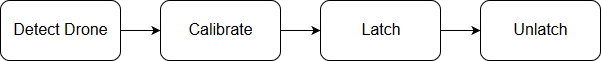
\includegraphics[width=\textwidth]{ProcessFlow}
	\caption{High Level Parts of Project}
	\label{fig:process}
\end{figure}

\begin{longtable} { |p{0.2\textwidth}|p{0.35\textwidth}|p{0.35\textwidth}| }	
	\hline
	\textbf{Step} & \textbf{Approach} & \textbf{Specification} \\
	\hline
	\underline{\textbf{Detect Drone}}\par\underline{\textbf{[Location]}}\par
	One drone must detect the location of another drone and travel within range for calibration and latching. 
	&
	\underline{Bluetooth}\par
	The two drones will have the ability to connect to each other through bluetooth automatically. This will allow them to share information to easily gain location information.\par\hfill\par 
	\underline{GPS}\par 
	The use of a GPS system will allow each drone to know its own location. Once each drone's location is known, bluetooth communication can be used to bring the drones closer to each other.\par\hfill\par 
	\underline{Barometer}\par 
	GPS is not accurate enough to measure height on a localized scale. Barometers will allow us to get the height of the drones to the right point for calibration.
	&
	\underline{Bluetooth}\par 
	Any bluetooth version newer than 1.2 will work as version 1.2 allowed fast discovery and connection.\par\hfill\par 
	\underline{GPS}\par 
	GPS is certified to an accuracy of 4 meters RMS. When combined with the barometer, this should allow the drones to get close enough for calibration.\par\hfill\par 
	\underline{Barometer}\par 
	Modern barometers can sense pressure differences in as little as a meter (or less) of height.
	Only the relative positions of the drones matter, so the barometer will be an easy way to make sure that one drone is higher than the other.\\
	\hline
	\underline{\textbf{Calibration}}\par
	Once the drones are in very close proximity to each other, they must come closer and align themselves for proper latching.			
	& 
	\underline{Vision Based Detection}\par
	Once the child drone detected the parent drone, they will be within several meters from each other. A camera on the child drone will be used to detect a special symbol on the parent drone.
	This allows the child drone to adjust its position such that the latching mechanisms are well-aligned. For example, consider the following symbol.
			
	\begin{center}
		
\includegraphics[width=5cm]{IdentificationExample}
	\end{center}

	Edge Detection can be done on this image in the following way:
	\begin{enumerate}
		\item Detecting the size of the triangle will allow the child drone to determine the distance from the parent drone, and move closer or farther, accordingly.
		\item Detecting the orientation of the arrow will allow the child drone to determine if it is facing the correct direction.
		\item The child drone is ready to latch when the front of the arrow lines up with the top of the edge detection frame. 
	\end{enumerate} 
	& 
	\underline{Hardware}\par
	To implement the computer vision based calibration, we will need to utilize a lightweight camera and make sure that there is enough room on the surface of the parent drone for a large, identifiable symbol.\par\hfill\par 
	We can also consider coloring the arms of the Parent drone in order to assist in getting the relative orientation before relying on the identification symbol.\par\hfill\par
	\underline{Software}\par
	In addition, because the drones move independently, we might need to account for the speed of the parent drone using computer vision.
	For example, we can use the number of pixels moved in a certain amount of time to determine how to adjust the child drone's speed to match that of the parent drone.\par\hfill\par 
	One potential approach that we may need to take, if a simple proportional navigation approach doesn't work, is to use the Extended Kalman Filter to control the thrust direction of the drone in proportion to the size and orientation of the symbol \cite{falanga2017ssrr}. \\
	\hline
	\underline{\textbf{Latching and}}\par\underline{\textbf{Unlatching}}\par
	Once the Child drone detects the Parent drone's location, moves near the Parent drone, and aligns its location above the Parent drone correctly through calibration, it will descend onto the Parent drone.
	The Child drone will be latched onto the Parent drone to prevent movement after landing.
	When the Child drone wants to take off again, the latch will be released and the Child drone will be free to fly away.
	&
	For latching, we thought of using electromagnets and regular magnets, as this would remove the need for additional mechanical parts and controls.
	There are two parts involved in latching the Child drone to the Parent drone.
	\begin{enumerate}
		\item Two electromagnets are fastened to the top of the Parent drone. We chose two electromagnets because 1) too many electromagnets will add too much weight to the Parent drone and 2) there should be enough space on the surface of the Parent drone for the identification symbol used in calibration. 
		\item There are regular magnets on the underside of the Child drone. When latching, the Parent drone's electromagnets will hold the Child drone in place. When unlatching, reversing the current that flows through the Parent drone's electromagnets should repel the magnets on the Child drone. 
	\end{enumerate}
	& 
	\underline{Electromagnets}\par 
	Electromagnets that have a 180 \si{\newton} peak force and 135 \si{\newton} holding force should be more than capable for the drone latching. One electromagnet that we can use is \href{https://www.amazon.com/uxcell-Electric-Lifting-Electromagnet-Solenoid/dp/B01MUA0ZLE}{uxcell 24V DC 180N Electric Lifting Magnet Electromagnet Solenoid Lift Holding}.\par\hfill\par
	\underline{Regular Magnets}\par
	Any regular circular magnet should be sufficient in holding the Child drone in place.\\
	\hline
	\caption{Details of Each Step in Our Design}
	\label{table:steps}
\end{longtable}
\newpage

\begin{figure}[h!]
	\centering
	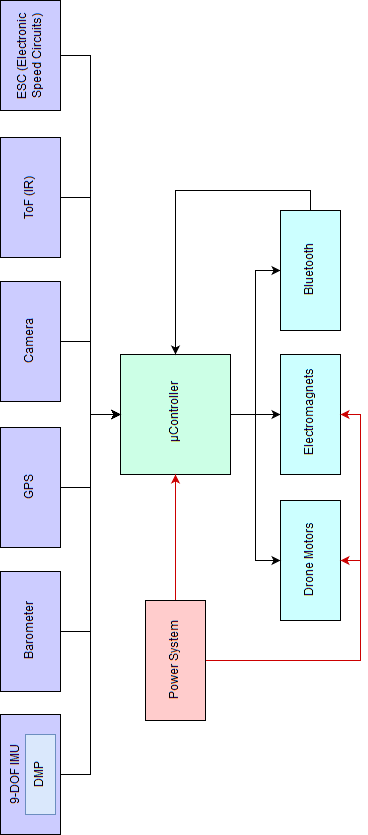
\includegraphics[width=0.57\textwidth]{BlockDiagram}
	\caption{High-level Block Diagram}
	\label{fig:prelimblockdiagram}
\end{figure}

\newpage
\section{Conceptual Drawings}
\begin{figure}[h]
	\centering
	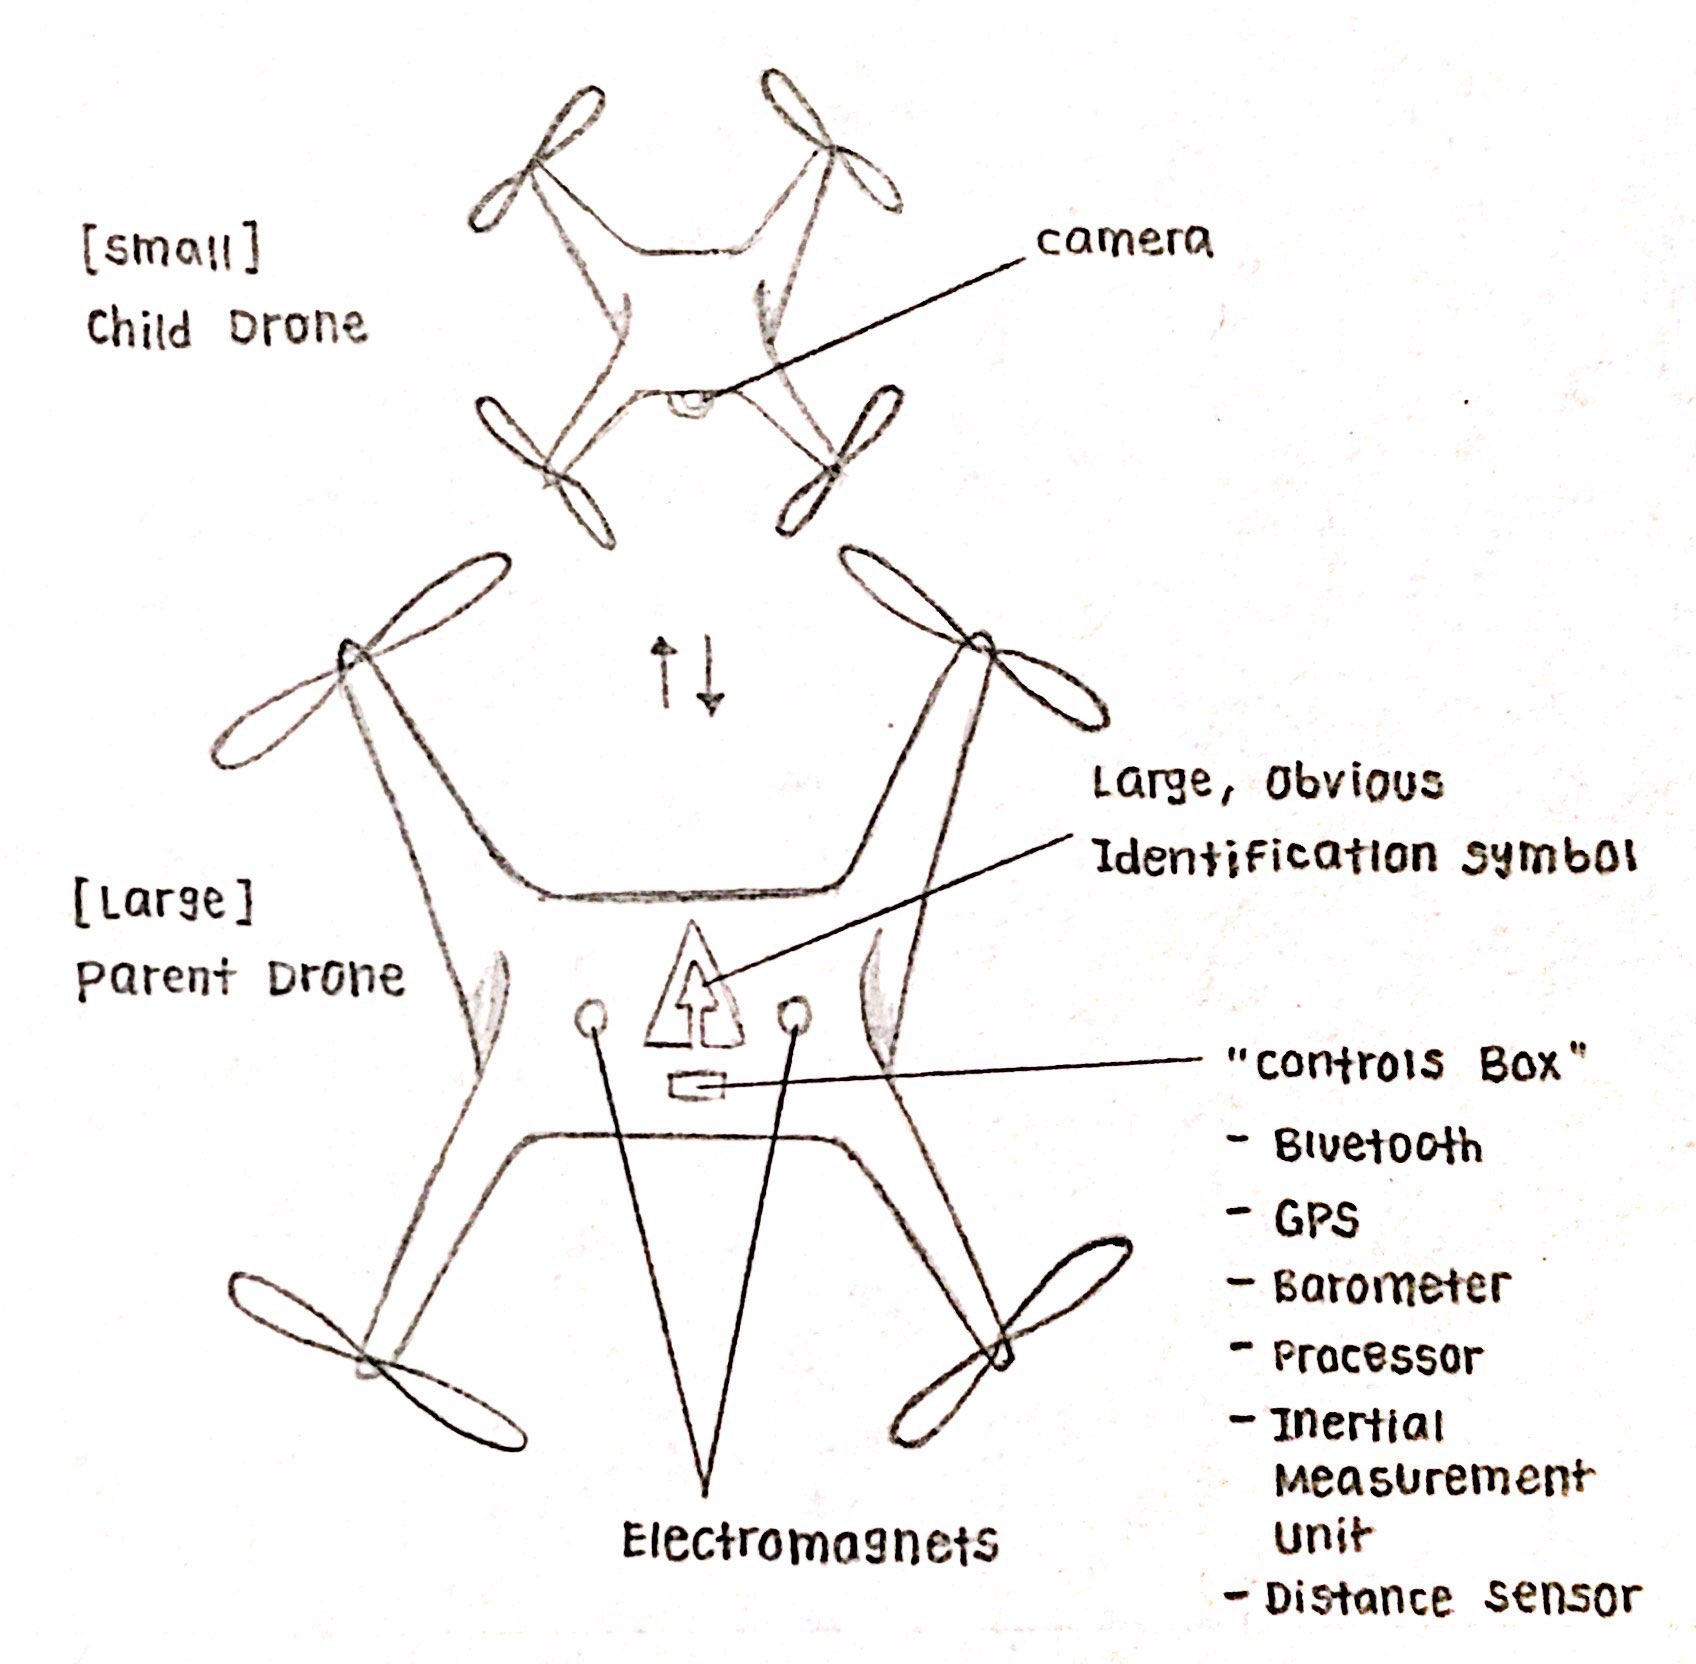
\includegraphics[width=0.57\textwidth]{ConceptDrawTopLevel}
	\caption{Top-level View of Entire System}
	\label{fig:toplevel}
\end{figure}

\begin{figure}[h]
	\centering
	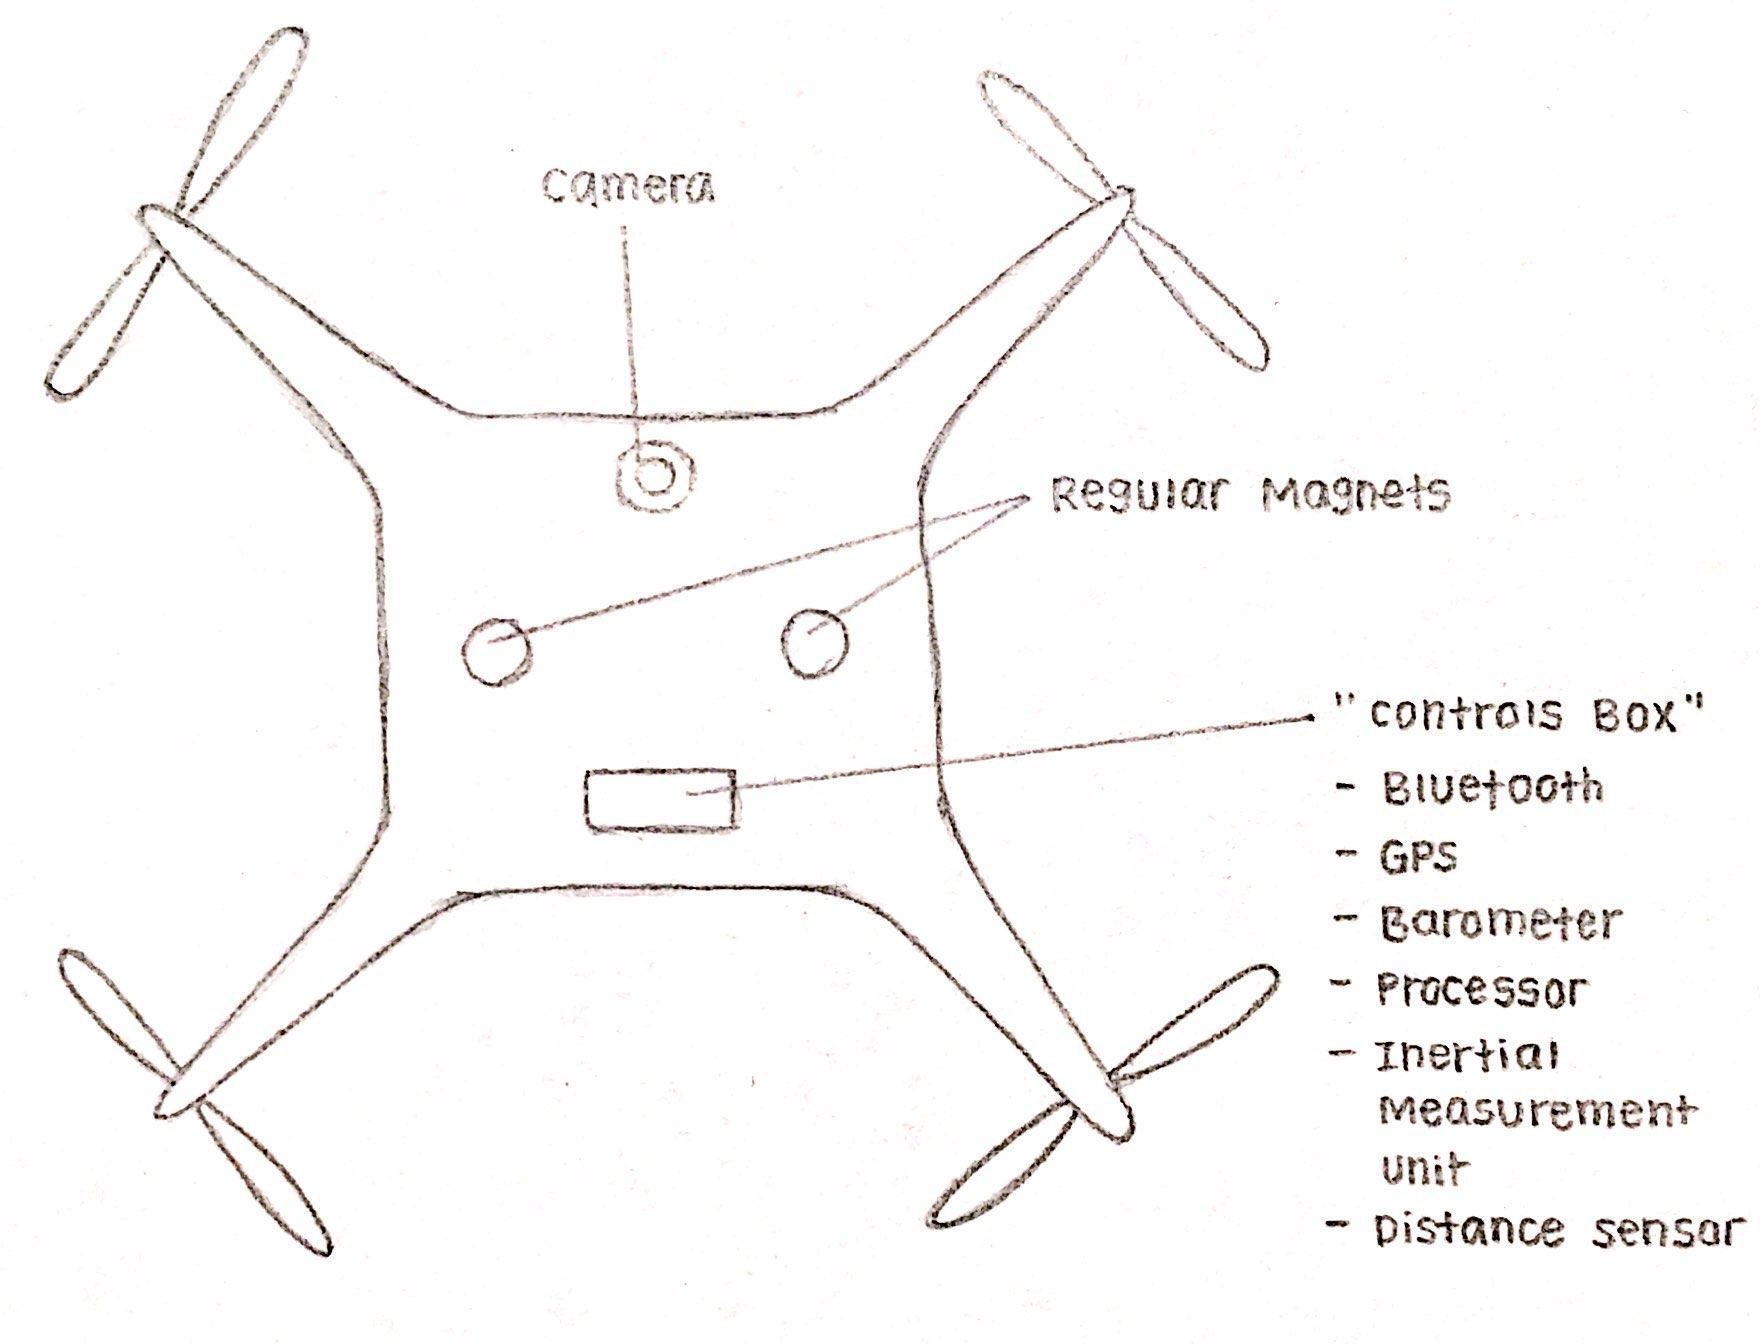
\includegraphics[width=0.57\textwidth]{ConceptDrawChildUnder}
	\caption{Underside of the Child Drone}
	\label{fig:childunderside}
\end{figure}

%%%%%%%%%%%%% END DOCUMENT CONTENT %%%%%%%%%%%%%

%%%%%%%%%%%%%%% BEGIN REFERENCES %%%%%%%%%%%%%%%
\bibliographystyle{ieeetr}
\bibliography{./bib/ref}
%%%%%%%%%%%%%%%% END REFERENCES %%%%%%%%%%%%%%%%

% End document
\end{document}